\section{Sintesi e caratterizzazione con 1H NMR di \ce{[Co(dinosar)]Cl3}}
\subsection{Sintesi \ce{[Co(en)3]Cl3}}
\subsubsection{Procedura sperimentale}
Abbiamo preparato una prima soluzione disciogliendo 6.02 g di \ce{CoCl2.6 H2O} in 17.5 mL circa d’acqua prelevata con un cilindro graduato. In contemporaneamente, abbiamo sciolto in un altro becher 5 mL (4.5 g) di etilendiammina in 12.5 mL di acqua. Quindi abbiamo acidificato la soluzione di etildiammina con 4.5 mL di acido cloridrico 6 M in un bagno di ghiaccio. Abbiamo unito le due soluzioni e abbiamo aspettato mezz’ora che avvenisse la complessazione. In seguito abbiamo aggiunto goccia a goccia 5.0 mL di acqua ossigenata al 30\% per ossidare il centro metallico. Al termine dell’effervescenza abbiamo svaporato a 30 mL e aggiunto lentamente 30 mL di HCl 12 M e 60 mL di etanolo. È precipitato un sale giallo ocra che abbiamo filtrato su Buchner, lavato con etanolo (3 × 10 mL). Abbiamo raccolto il prodotto in una provetta precedentemente pesata e l'abbiamo seccato sottovuoto.

\subsubsection{Commenti e osservazioni}
Durante l'acidificazione dell'etildiammina con HCl abbiamo notato la formazione di fumi bianchi. Questi si presume dovuti all'etildiammonio cloruro prodotto dalla reazione dell'acido cloridrico gassoso con etildiammina passata in fase gas per il riscaldamento della soluzione dovuto all'esotermicità della reazione di acidificazione. L'acqua ossigenata utilizzata era stata tenuta in frigo, i perossidi sono sostanze sensibili e tendono a decomporsi.


\subsubsection{Calcoli e analisi dei dati}
In partenza avevamo un numero di moli di reagenti pari a
$$
\begin{gathered}
n_{\mathrm{CoCl}_2}=\frac{6.00 \mathrm{~g}}{237.93 \mathrm{~g} / \mathrm{mol}}=0.0253 \mathrm{~mol} \\
n_{\mathrm{en}}=\frac{5 \mathrm{~mL} \cdot 0.899 \mathrm{~g} / \mathrm{mL}}{60.10 \mathrm{~g} / \mathrm{mol}}=0.07479 \mathrm{~mol}
\end{gathered}
$$
La stechiometria della reazione è 1 : 3 notiamo che il reagente limitante è l'etilendiammina\footnote{E' il reagente limitante per poco. }.
Calcoliamo la resa 
\[ Y_\% = \frac{n_\text{pro}}{n_{\mathrm{CoCl}_2}}\cdot 100 \]

Le moli finali sono il rapporto massa della provettà piena di prodotto tolta la tara e la massa molare del prodotto.

\[ n_\text{pro} = \frac{(m_{f\#1} - m_{t\#1})+(m_{f\#2} - m_{t\#2})}{M_\text{pro}} 
 = \frac{ 3.7564 \um{g} + 4.1124 \um{g} }{ 345.58 \um{g/mol}} =  \frac{7.8688 \mathrm{~g}}{345.58 \mathrm{~g} / \mathrm{mol}}=22.77 \um{mmol}\]

\[ Y_\% = \frac{n_\text{pro}}{n_{en}}\cdot 100  = \frac{3 \cdot 22.77 \cdot 10^{-3} \mathrm{~mol}}{74.79 \cdot 10^{-3} \mathrm{~mol}} \cdot 100 =91.3\%\]


\subsection{Sintesi \ce{[Co(dinosar)]Cl3}}
\subsubsection{Procedura sperimentale}
Abbiamo sciolto $2.45 \mathrm{~g}$ esatti del prodotto del passaggio precedente in $25 \mathrm{~mL}$ di acqua con $1.20 \mathrm{~g}$ di carbonato di sodio. Abbiamo quindi aggiunto $18 \mathrm{~mL}$ di formaldeide al $40 \%$ prelevata con un cilindro e $2.5 \mathrm{~mL}$ (circa $2.8 \mathrm{~g}$) di nitrometano. Dopo aver lasciato la soluzione a temperatura ambiente per qualche ora l'abbiamo riscaldata per un'altra ora al minimo della piastra elettrica. Abbiamo quindi filtrato su Buchner e recuperato il precipitato arancione che abbiamo ricristallizzato da una soluzione in $\mathrm{HCl} $ 3M. Infine, dopo aver aggiunto etanolo come non solvente abbiamo filtrato su Buchner, seccato all'aria, trasferito in una provetta di massa nota e seccato sottovuoto.
\subsubsection{Commenti e osservazioni}
Non sono stati notati significativi eventi degni di essere riportati.


\subsubsection{Calcoli e analisi dei dati}
In partenza avevamo un numero di moli di reagenti pari a
\[ n_{\ce{[Co(en)3]Cl3}}=\frac{2.45 \mathrm{~g}}{345.58 \mathrm{~g} / \mathrm{mol}}= 7.090 \mathrm{~mmol} \]

\[ n_{\mathrm{HCOH}}=\frac{18 \mathrm{~mL} \cdot 1.09 \mathrm{~g} / \mathrm{mL} \cdot 40 \%}{30.03 \mathrm{~g} / \mathrm{mol}}=0.26 \mathrm{~mol} \]
\[ n_{\mathrm{CH}_3 \mathrm{NO}_2}=\frac{2.5 \mathrm{~mL} \cdot 1.127 \mathrm{~g} / \mathrm{mL}}{61.04 \mathrm{~g} / \mathrm{mol}}=0.0462 \mathrm{~mol} \]

Considerando quindi la stechiometria $1: 6: 2$ notiamo che il complesso il reagente limitante. Abbiamo ottenuto $ 2.675 \mathrm{~g}$ di prodotto



Calcoliamo la resa 
\[ Y_\% = \frac{n_\text{pro}}{n_{\ce{[Co(en)3]Cl3}}}\cdot 100 \]

Le moli finali sono il rapporto massa della provettà piena di prodotto tolta la tara e la massa molare del prodotto.

\[ n_\text{pro} = \frac{(m_{f} - m_{t})}{M_\text{pro}} 
 = \frac{ 17.7611 \um{g} - 15.0861 \um{g} }{ 539.73 \um{g/mol}} =  \frac{2.675 \mathrm{~g}}{539.73 \mathrm{~g} / \mathrm{mol}}=4.96 \um{mmol}\]

\[ Y_\% = \frac{n_\text{pro}}{n_{\ce{[Co(en)3]Cl3}}}\cdot 100  = \frac{ \cdot 4.96 \cdot 10^{-3} \mathrm{~mol}}{7.09 \cdot 10^{-3} \mathrm{~mol}} \cdot 100 =70.0\%\]

\subsection{Spettro NMR}



\begin{figure}
    \centering
    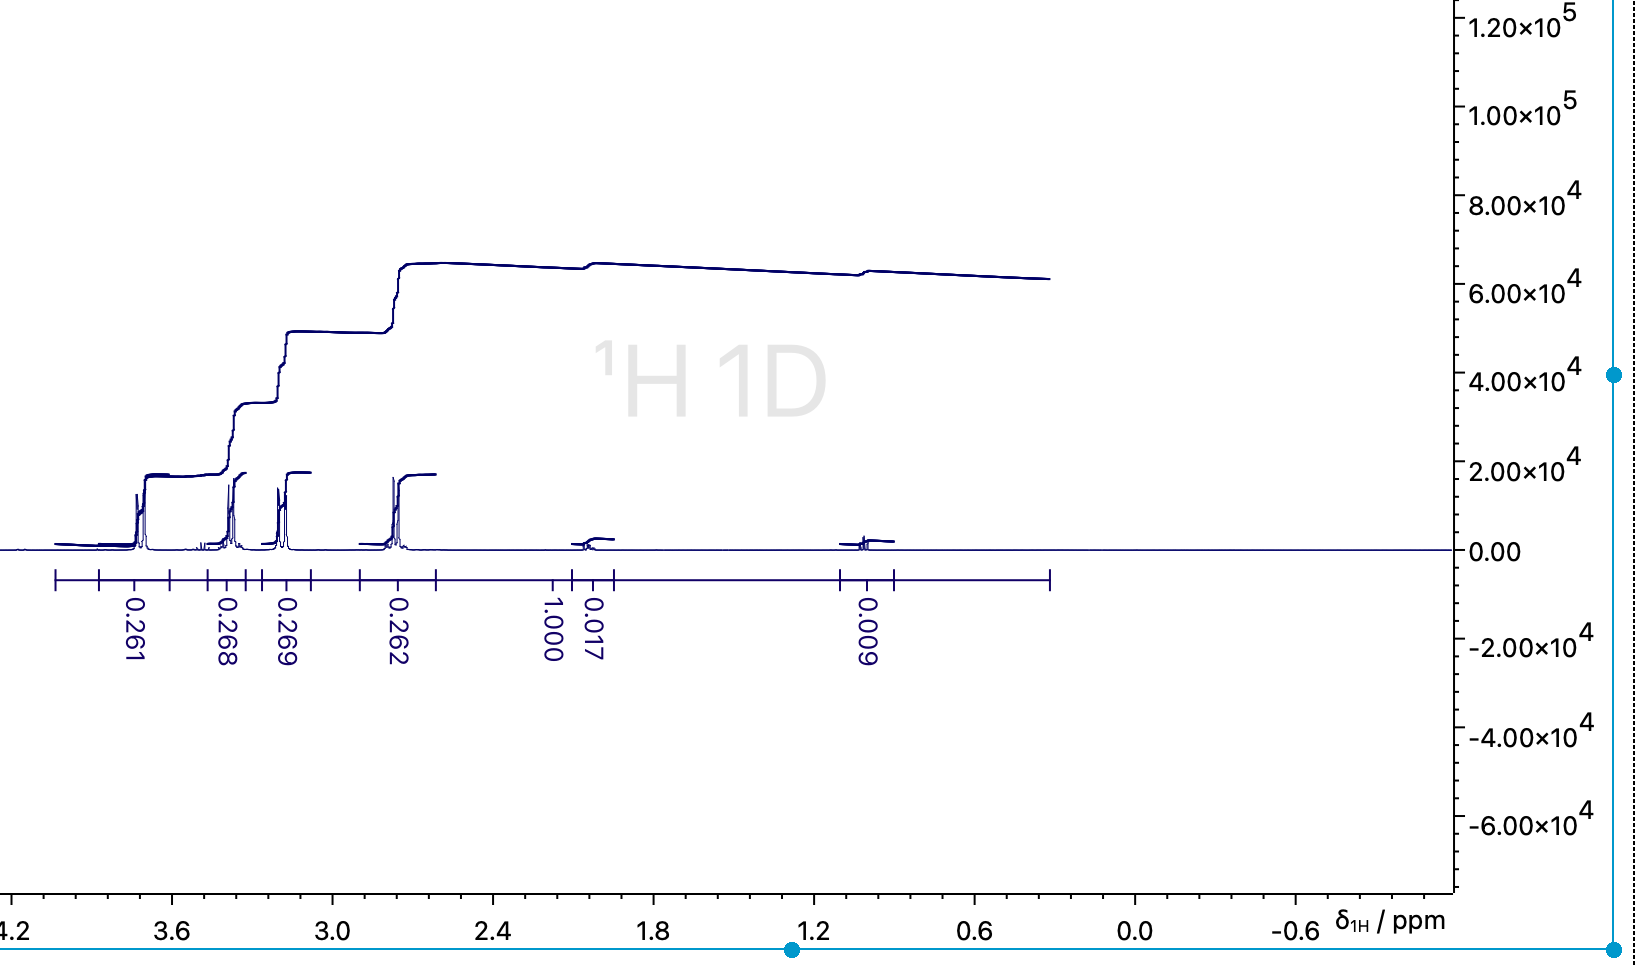
\includegraphics[width=0.8\linewidth]{Relazione/foto/Dinosar_integration_zoom.png}
    \caption{Spettro Co(dinosar) integrato.}
    \label{fig:dinosarint}
\end{figure}



\begin{figure}
    \centering
    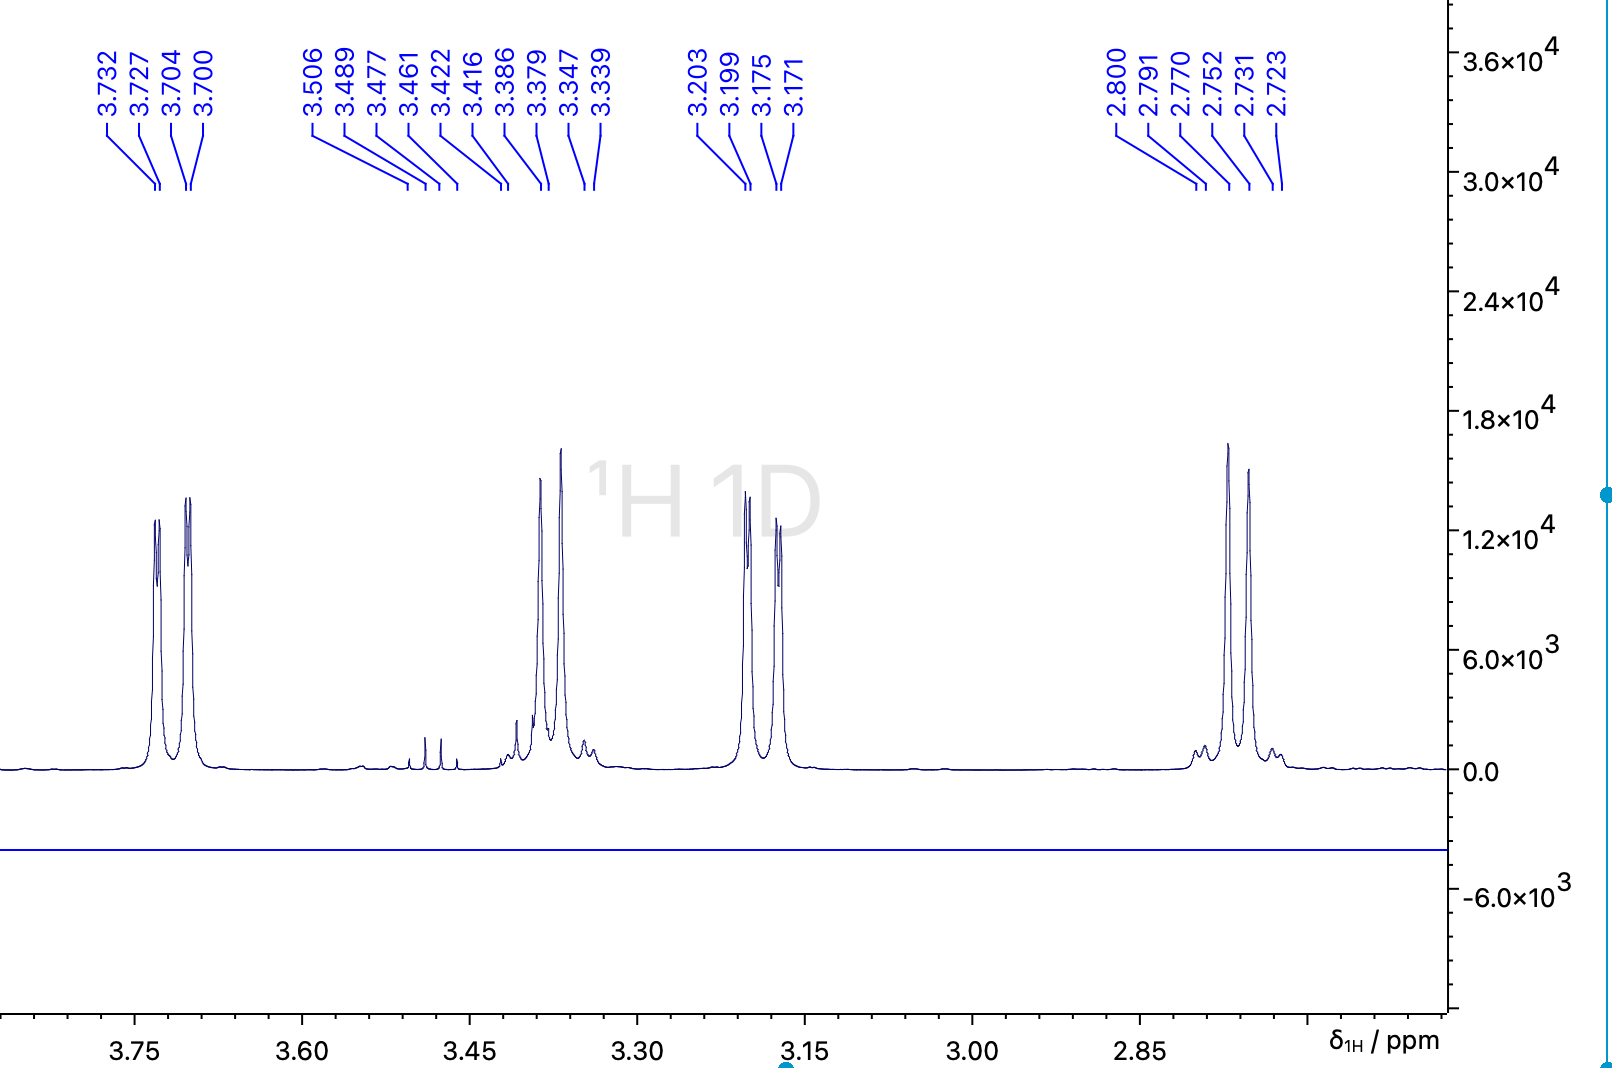
\includegraphics[width=0.8\linewidth]{Relazione/foto/Dinosar_peak_calc.png}
    \caption{Spettro Co(dinosar), con assegnazione dei picchi.}
    \label{fig:dinosarpeakcalc}
\end{figure}
Nello spettro si possono riconoscere 4 picchi relativi a 4 gruppi di idrogeni non equivalenti, possiamo inoltre notare anche 3  piccoli picchi che possono essere dovuti all'etanolo rimasto dopo il lavaggio (3.5 ppm e 1 ppm, il picco a 2 ppm può essere dovuto a qualche inquinante incognito). Senza considerare la pro-chiralità della molecola possiamo categorizzare gli idrogeni in due categorie, l'idrogeni in $\beta$ al gruppo nitro e gli idrogeni relativi alla etilendiammina, notare che lo spettro è stato misurato in \ce{D2O} quindi l'idrogeni collegati all'azoto non vengono rilevati in quanto sono attivi per lo scambio isotopico con il solvente. Teniamo presente che entrambi sono protoni diastereotopici, quindi otterremo  4 tipi di protoni equivalenti. In \autoref{fig:protodino} è mostrata una schematizzazione della molecola e degli idrogeni relativi ai picchi NMR. Potremo già attribuire a priori \ce{H1} e \ce{H2} ai picchi a 3.7 ppm e 3.2 ppm in quando gli effetti induttivi rendono il centro ai cui sono collegati i due idrogeni più elettron-povero rispetto all'altro. Il picco a 3.2 ppm è ovviamente associato a quello a 3.7 ppm in quanto hanno la stessa forma, questo implica che in teoria associano nello stesso modo. Possiamo confermare questa assunzione dal profilo dei picchi e dalla molteplicità, infatti se prendiamo per esempio \ce{H1} esso accoppia ${}^2$J con \ce{H2}, questo è indice di una rigidità strutturale del Co(dinosar) che viene confermata dalla presenza di una costante ${}^4$J che separa ulteriormente i picchi, anche se in misura molto minore.
\begin{figure}[h!]
    \centering
    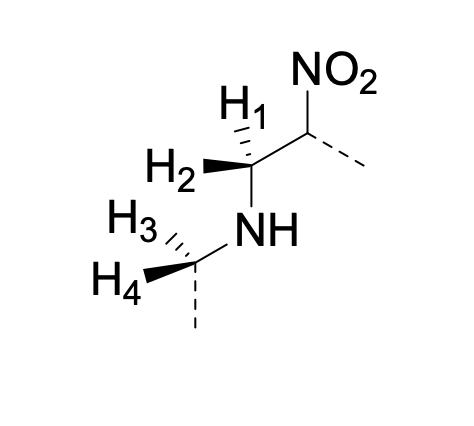
\includegraphics[width=0.3\linewidth]{Relazione/foto/protonidino.png}
    \caption{Protoni non equivalenti del Co(dinosar)}
    \label{fig:protodino}
\end{figure}

La separazione in chemical shift tra \ce{H1} e \ce{H2} che è circa 0.5 ppm, concorda con la separazione tra idrogeni equatoriali e assiali nei sistemi in cui la libera rotazione è impedita. Questo fenomeno è dovuto dall'anisotropia magnetica derivante dal legame C-C. Per \ce{H3} e \ce{H4} i ragionamenti sono pressoché analoghi tranne per il fatto che in questo caso sono presenti anche due accopiamenti ${}^3$J circa equivalenti che creano in unione a ${}^2$J un sestupletto. Non è presente l'accoppiamento ${}^4$J.

